\section{Java Business Integration}
\label{sec:jbi}

The interaction between enterprises' applications has suffered in the past from lack of standardized technologies, leading each of the enterprises to develop their own or acquiring vendor-specific integration technology. \ac{JBI} is defined by the Java Community as an integration technology which maximizes the decoupling between components and defines an interoperation semantic founded on standards-based messaging. This allows different vendor-specific components to interoperate in a multivendor "echosystem" \cite{JBI2005}. 

The key which leads to the integration of different components relies on a unique message format in the \ac{JBI} environment which different plugged-in components use to communicate within the environment. External components are not directly connected, but through a mediator. The communication mediator between components in a \ac{JBI} environment is the \ac{NMR}. Its main functionality is the routing of the internal standardized \ac{NM} between the components. However, it can perform additional processing during the message exchange. The \ac{NMR} fields are defined as an \ac{XML} document format payload, metadata conforming the header and a non \ac{XML} document format attachment referenced by the payload.

The \ac{JBI} specification defines two different types of components which are categorized in two types and provide different services:
	\begin{itemize}
		\item A \ac{SE} provides transformation and composition services to other components.
		\item A \ac{BC} provides the connectivity between the external services and the \ac{JBI} environment. They support many different protocols and isolate the \ac{JBI} environment by marshaling and demarshaling the incoming or outgoing message into the internal standardized \ac{NM} format.
	\end{itemize} 
	
Both components listed above can function as service consumers or service providers following a \ac{WSDL}-based, service-oriented model. The consumer endpoint provides a service accessible through an endpoint which can be consumed by other components, while the provider endpoint consumes a functionality exposed as a service and accessible through an external endpoint. The routing of \ac{NM} starts when a message exchange between components is created (bidirectional communication pipe, a \term{DeliveryChannel}, between the communicating endpoints) and continues with the target of the specified service endpoint for processing (see Figure \ref{fig:jbi}). The \ac{NMR} supports four asynchronous message exchange patterns differing in the reliability and direction of the communication.

\begin{figure}[htb]
	\centering
		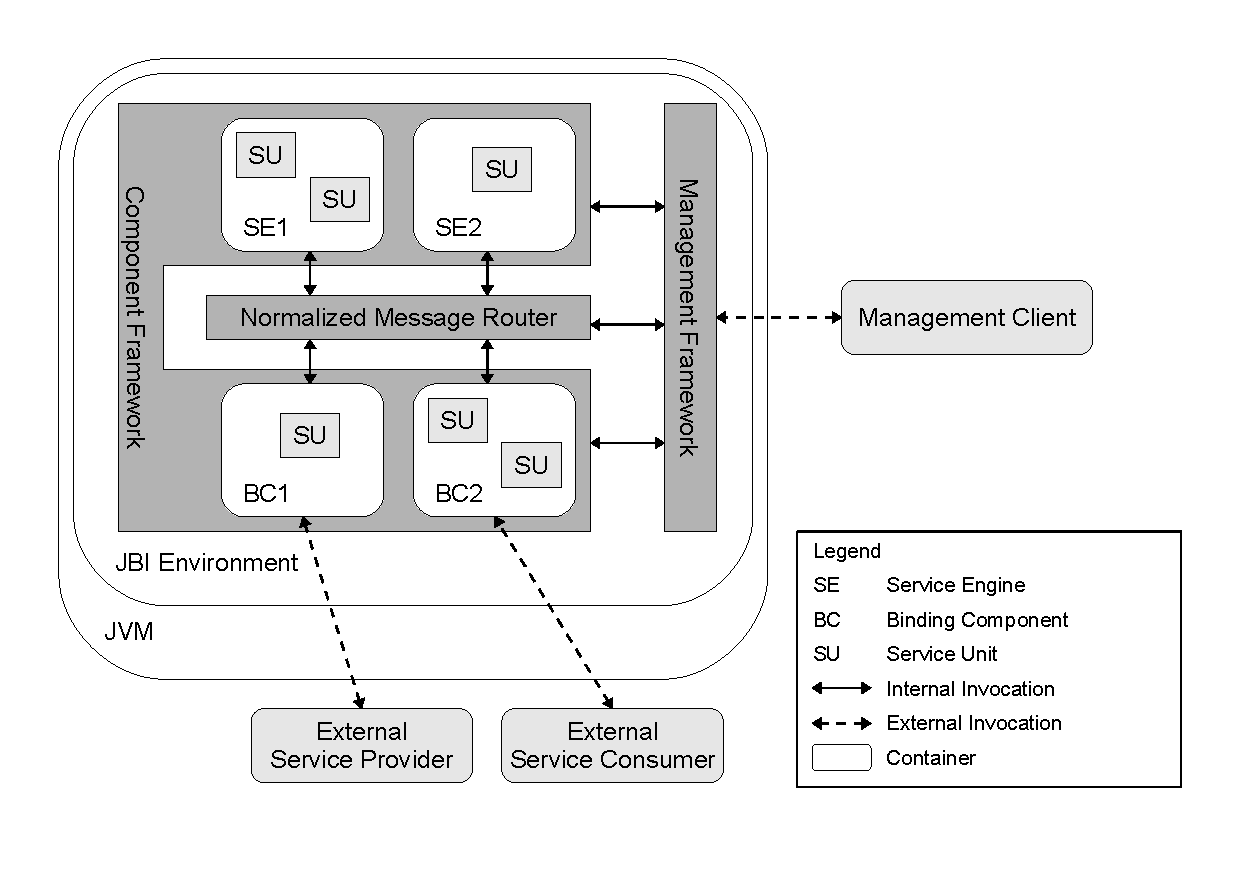
\includegraphics[width=0.85\textwidth, trim=0.95cm 0.95cm 0.95cm 0.95cm, clip]{./gfx/JBIArchitecture.pdf}
	\caption[JBI Architecture]{Overview of JBI Architecture. Figure 4 in JBI specification document \cite{JBI2005}.}
	\label{fig:jbi}
\end{figure}

In Figure \ref{fig:jbi} we can observe that one or more \ac{SU} are contained in a \ac{BC}. The \ac{SU}s are component-specific artifacts to be installed to a \ac{SE} or a \ac{BC} \cite{JBI2005}. The service units are packed in a \ac{SA}, usually as ZIP files, where it is specified each of the components where each of the \ac{SU}s should be deployed. The \ac{JBI} environment provides a Java Management Extension \ac{JMX} Framework for installation, life cycle management, addition, and monitoring and control of the components conforming to the environment defined by the JBI specification.

\FloatBarrier